\documentclass[10pt,a4paper]{article}
\usepackage[T1]{fontenc}
\usepackage[utf8]{inputenc}
\usepackage{lmodern}
\usepackage[scaled=0.92]{helvet}
\renewcommand{\familydefault}{\sfdefault}
\usepackage{microtype}
\usepackage[a4paper,margin=1.8cm,top=1.6cm,bottom=1.8cm]{geometry}
\usepackage{graphicx}
\usepackage{booktabs}
\usepackage{tabularx}
\usepackage{xcolor}
\usepackage{caption}
\usepackage{subcaption}
\usepackage{enumitem}
\usepackage{titlesec}
\usepackage{fancyhdr}
\usepackage{pgfplots}
\pgfplotsset{compat=1.17}
\usepackage[hidelinks]{hyperref}

\definecolor{leaf}{HTML}{2E6B4A}
\definecolor{soil}{HTML}{6B4A2E}
\definecolor{ink}{HTML}{1C2520}
\definecolor{muted}{HTML}{5D6A62}
\definecolor{band}{HTML}{E8F0EA}
\definecolor{warn}{HTML}{B8422A}

\color{ink}
\titleformat{\section}{\large\bfseries\color{leaf}}{\thesection}{0.6em}{}
\titleformat{\subsection}{\normalsize\bfseries}{\thesubsection}{0.5em}{}
\titlespacing*{\section}{0pt}{10pt}{4pt}
\titlespacing*{\subsection}{0pt}{6pt}{2pt}
\captionsetup{font=small,labelfont={bf,color=leaf},skip=4pt}
\captionsetup[sub]{font=footnotesize,skip=2pt}
\setlist{nosep,leftmargin=1.2em}
\setlength{\parindent}{0pt}
\setlength{\parskip}{4pt}
\renewcommand{\arraystretch}{1.12}

\pagestyle{fancy}
\fancyhf{}
\renewcommand{\headrulewidth}{0pt}
\fancyfoot[L]{\footnotesize\color{muted}Nabta project report · 23 November 2026}
\fancyfoot[R]{\footnotesize\color{muted}\thepage}

\begin{document}

%-------------------------------------------------------------- title
{\color{leaf}\fontsize{24}{28}\selectfont\bfseries Nabta}\par\vspace{2pt}
{\large An offline AI smart pot for spearmint: project report}\par\vspace{3pt}
{\small\color{muted}Nabta team · CS496 AI Engineering · MedTech · 23 November 2026 ·
Code and designs: \href{https://github.com/Ahmed-Hammoda/nabta}{github.com/Ahmed-Hammoda/nabta}}

\vspace{6pt}
\colorbox{band}{\parbox{\dimexpr\textwidth-2\fboxsep}{\small
\textbf{Summary.} Nabta looks after one jar of spearmint with a soil probe, a light sensor and an air
temperature/humidity sensor on a Raspberry Pi~4 (4~GB), with no internet. We tested whether a small
language model can run the pot. It cannot do so safely: across 35 model–prompt runs on a simulated
30-day log, the best run had both water and alerts right in only 63\,\% of cases and still watered a
broken sensor. So in the final system \textbf{fixed rules decide, and the model only explains}.
qwen3.5:0.8b explains each decision (all 184 test explanations agreed with the rules) and answers
questions (231 of 240 chat answers passed every check). The sensors, rules, logging and pump
safety run on the Pi; a phone app and a 3D-printed sensor stake are built.}}

%-------------------------------------------------------------- 1
\section{System}

\begin{figure}[h]
\centering
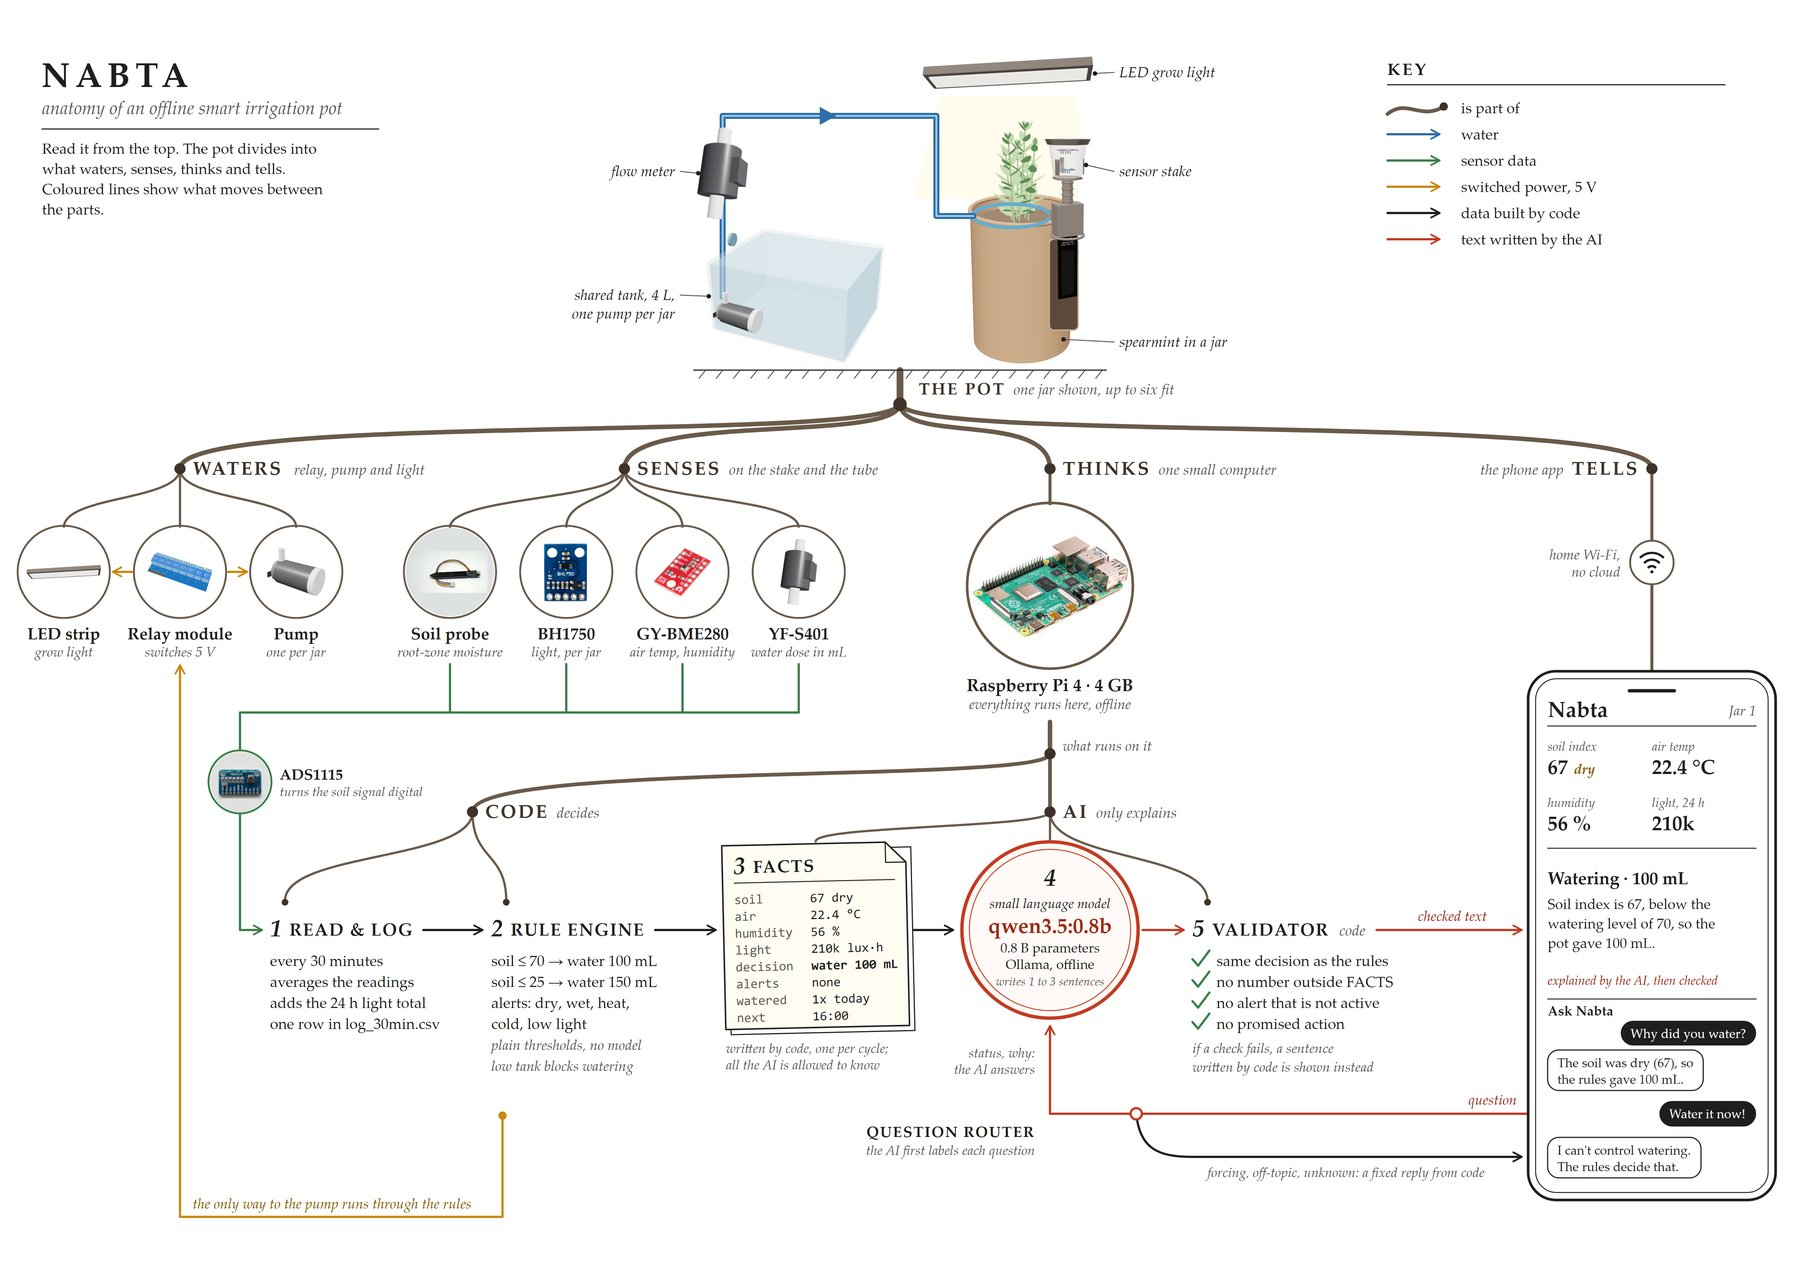
\includegraphics[width=\textwidth]{img/system_diagram.jpg}
\caption{The Nabta system. Code reads the sensors every 30 minutes and decides; the language model
only writes the explanation, and code checks it before the app shows it. (The flow meter drawn here
was later dropped: the water dose is now set by the pump's run time.)}
\end{figure}

Every 30 minutes the Pi averages the readings and turns the soil signal into a 0--100 index
(air = 0, water = 100). The rules first check for faults (broken or unplugged sensor, impossible
values, a pump that runs on its own), then decide: \textbf{water when the soil index is 70 or below},
and raise alerts for danger-dry soil ($\le$\,25), too wet ($\ge$\,98), heat ($>$\,36\,$^\circ$C),
cold ($<$\,4\,$^\circ$C) and low light ($<$\,90{,}000 lux·h per day). The temperature limits follow
FAO ECOCROP; all limits and their sources are listed in the repository.

%-------------------------------------------------------------- 2
\section{Hardware prototype}

\begin{figure}[h]
\centering
\begin{subfigure}[t]{0.415\textwidth}\centering
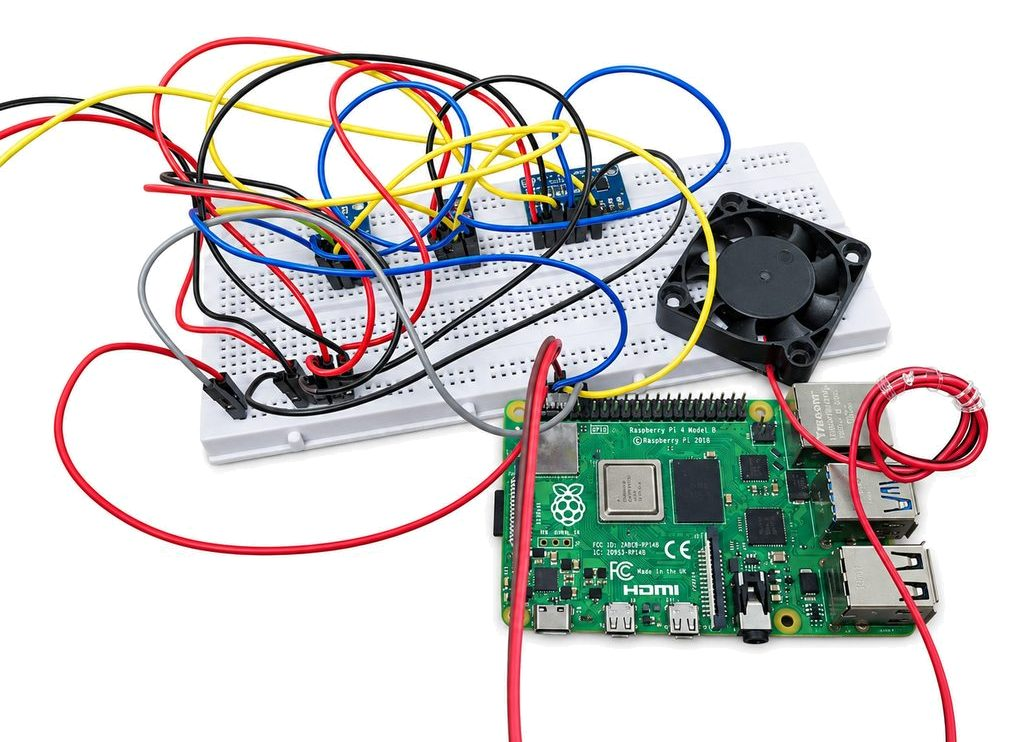
\includegraphics[height=5.1cm]{img/pi_prototype.jpg}
\caption{Raspberry Pi 4, sensors and fan}
\end{subfigure}\hfill
\begin{subfigure}[t]{0.235\textwidth}\centering
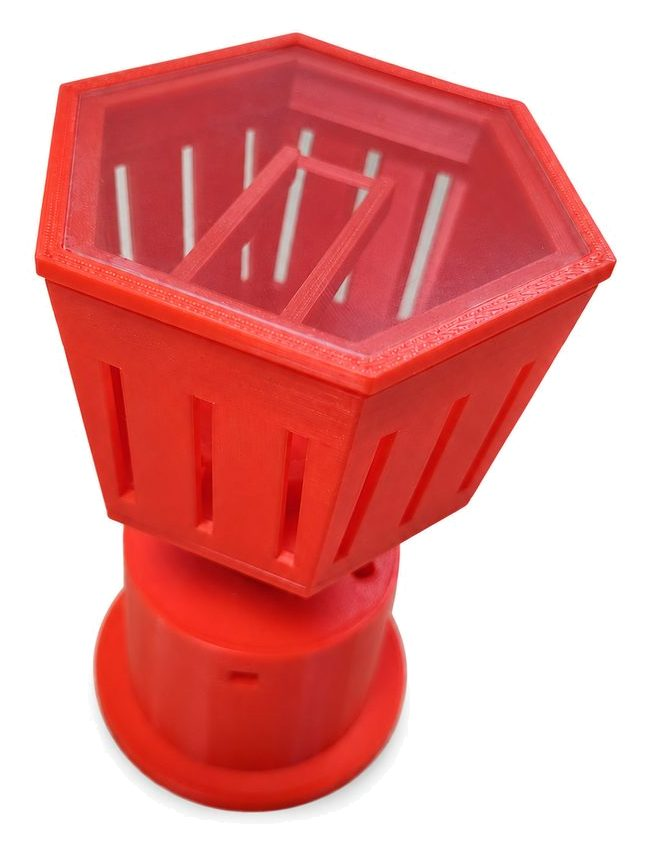
\includegraphics[height=5.1cm]{img/sensor_stake.jpg}
\caption{Printed sensor stake}
\end{subfigure}\hfill
\begin{subfigure}[t]{0.30\textwidth}\centering
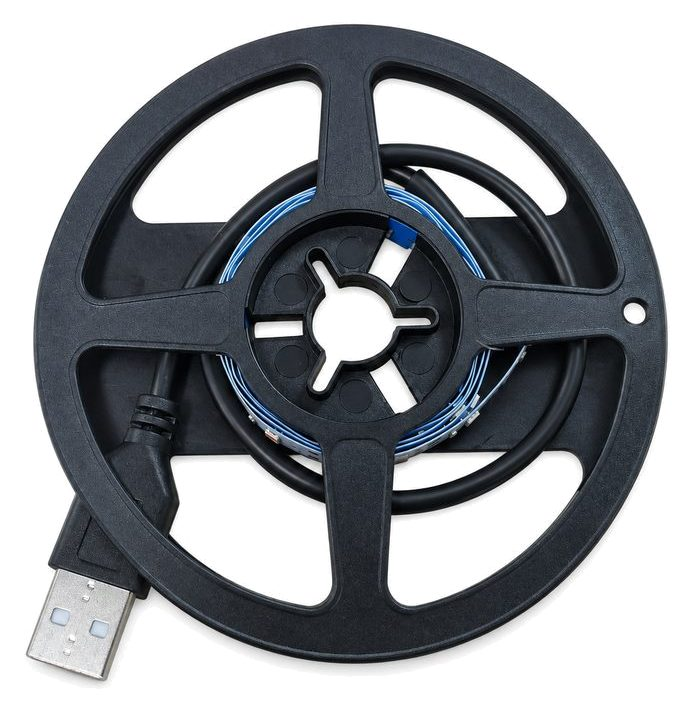
\includegraphics[height=5.1cm]{img/grow_light.jpg}
\caption{USB 5\,V grow-light strip}
\end{subfigure}
\caption{The prototype parts.}
\end{figure}

\begin{tabularx}{\textwidth}{@{}lX@{}}
\toprule
\textbf{Part} & \textbf{Role} \\
\midrule
Raspberry Pi 4, 4 GB & Runs the logger, the rules, Ollama with the model, and the chat; no cloud \\
Capacitive soil probe + ADS1115 & Soil moisture; calibrated in air (raw 16,700 $\to$ 0) and water (raw 7,887 $\to$ 100) \\
BH1750 / BME280 & Light (lux, summed over 24 h) / air temperature and humidity, both on the I$^2$C bus \\
Sensor stake (3D printed) & Holds the probe in the root zone and both sensors among the leaves \\
2-relay module, USB pump, float switch & Pump (relay 1), grow light (relay 2), tank-low signal; wiring designed \\
\bottomrule
\end{tabularx}

%-------------------------------------------------------------- 3
\section{Can a small language model run the pot?}

\subsection{Deciding: no}

\textbf{Phase 1} (184 hand-built cases): given raw numbers, no small model decided reliably.
qwen2.5:0.5B and gemma3:1b gave the same answer for every pot; qwen3.5:0.8b reached 83\,\% on the
water decision. Models only scored well when code had already computed the levels for them, which
means the code was doing the decision. Five lines of rule code get 100\,\%.

\textbf{Phase 2} (simulated 30-day log, 1,440 rows; 255 test cases including 10 sensor- or pump-fault rows):
5 models $\times$ 7 prompts = 35 runs. \emph{Both correct} means the water decision and every
alert are right.

\begin{minipage}[t]{0.56\textwidth}
\vspace{0pt}
\small
\begin{tabularx}{\linewidth}{@{}Xrrrc@{}}
\toprule
Model + prompt & Both & Water & Alerts & Fault rows watered \\
\midrule
qwen3:1.7b v3 & 63.3 & 86.1 & 68.6 & \color{warn}8/10 \\
lfm3:1.7b v3 & 49.0 & 98.4 & 49.8 & \color{warn}8/10 \\
lfm3:1.7b p5 (best safe run) & 47.8 & 91.8 & 49.4 & 0/10 \\
Do nothing (baseline) & 23.7 & 83.7 & -- & 0/10 \\
\bottomrule
\end{tabularx}\par
\footnotesize\color{muted} Values in \%. 25 of the 35 runs scored below the do-nothing baseline.
\end{minipage}\hfill
\begin{minipage}[t]{0.41\textwidth}
\vspace{0pt}
\centering
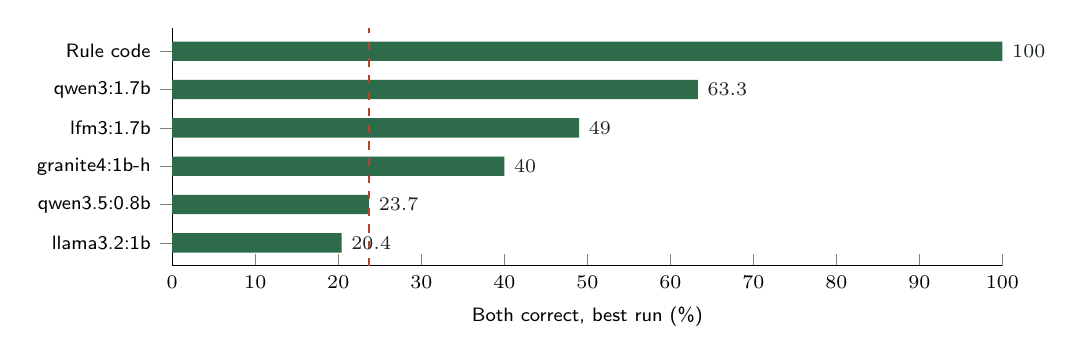
\begin{tikzpicture}
\begin{axis}[
  xbar, width=\linewidth, height=4.6cm, bar width=7pt,
  xmin=0, xmax=100, xlabel={Both correct, best run (\%)}, xlabel style={font=\scriptsize},
  symbolic y coords={llama3.2:1b,qwen3.5:0.8b,granite4:1b-h,lfm3:1.7b,qwen3:1.7b,Rule code},
  ytick=data, yticklabel style={font=\scriptsize}, xticklabel style={font=\scriptsize},
  nodes near coords, nodes near coords style={font=\scriptsize, color=ink}, enlarge y limits=0.12,
  axis lines*=left, every axis plot/.append style={fill=leaf, draw=none}]
\addplot[fill=leaf, draw=none] coordinates {(20.4,llama3.2:1b) (23.7,qwen3.5:0.8b) (40.0,granite4:1b-h) (49.0,lfm3:1.7b) (63.3,qwen3:1.7b) (100,Rule code)};
\draw[warn, dashed, thick] ({rel axis cs:0,0} -| {axis cs:23.7,qwen3:1.7b}) -- ({rel axis cs:0,1} -| {axis cs:23.7,qwen3:1.7b});
\end{axis}
\end{tikzpicture}\par
\footnotesize\color{muted} Dashed: do-nothing baseline (23.7\,\%).
\end{minipage}

Turning on \emph{thinking} raised qwen3:1.7b from 29.9\,\% to 51.9\,\% both-correct on 82 cases,
but each answer took 13 times longer (6.5\,s on the laptop GPU), and lfm3:1.7b's thinking runs did not
finish. \textbf{Conclusion: no model is safe enough to control the pump}, so the rules decide.

\subsection{Explaining and chatting: yes}

\begin{minipage}[t]{0.52\textwidth}
\vspace{0pt}
qwen3.5:0.8b was tested on explaining the rule decision (184 cases, prompt e3):

\small
\begin{tabularx}{\linewidth}{@{}Xr@{}}
\toprule
Check (automatic) & Passed \\
\midrule
Same action as the rules & 100\,\% \\
No invented numbers & 100\,\% \\
Every active alert mentioned & 100\,\% \\
No fake alert & 99.5\,\% \\
Short (2 sentences, 40 words) & 98.4\,\% \\
\bottomrule
\end{tabularx}\par
\normalsize
A manual read found 2 real errors in 184; a 30-answer human check passed.
\end{minipage}\hfill
\begin{minipage}[t]{0.44\textwidth}
\vspace{0pt}
\centering
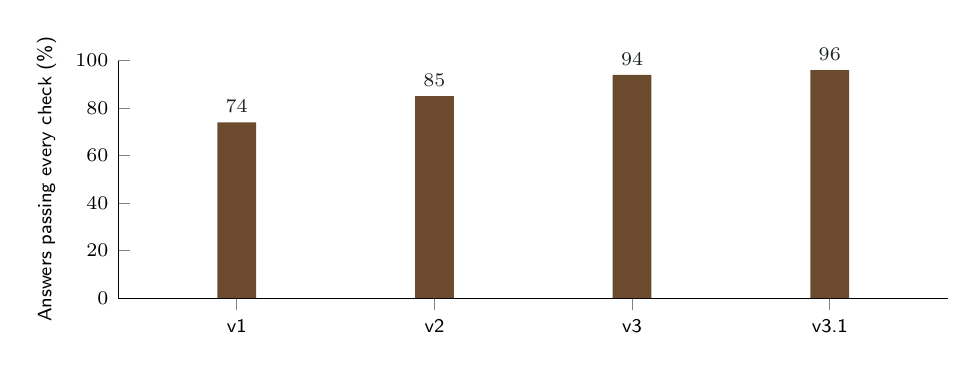
\begin{tikzpicture}
\begin{axis}[
  ybar, width=\linewidth, height=4.6cm, bar width=14pt,
  ymin=0, ymax=100, ylabel={Answers passing every check (\%)}, ylabel style={font=\scriptsize},
  symbolic x coords={v1,v2,v3,v3.1}, xtick=data,
  xticklabel style={font=\scriptsize}, yticklabel style={font=\scriptsize},
  nodes near coords, nodes near coords style={font=\scriptsize, color=ink}, enlarge x limits=0.2,
  axis lines*=left, every axis plot/.append style={fill=soil, draw=none}]
\addplot[fill=soil, draw=none] coordinates {(v1,74) (v2,85) (v3,94) (v3.1,96)};
\end{axis}
\end{tikzpicture}\par
\footnotesize\color{muted} Chat, 240 answers (40 questions $\times$ 6 plant situations).
\end{minipage}

The chat reached 96\,\% after adding a question router (the model sorts the question; forcing,
off-topic and unknown questions get a fixed reply written by code), facts built by code, and a safety
net that replaces a bad answer. It never contradicted the decision, invented a number, raised a fake
alert or promised an action. These prompts were tuned on the same 40 questions, so a fresh set of
questions is still needed to confirm the score.

\textbf{Fine-tuning} qwen3.5:0.8b to make the decision itself is prepared but not run: 6,600 labelled
rows plus 1,553 explanation ``replay'' rows (so it keeps its explaining skill), and a Colab notebook.

%-------------------------------------------------------------- 4
\section{The system running on the Raspberry Pi}

The logger, the rules and the controller run as services that start at boot. Readings and decisions
go into monthly folders that survive power cuts. The pump has three safety locks: no second watering
within 3 hours, at most 3 a day, and never on a reading more than 45 minutes old.

\begin{tabularx}{\textwidth}{@{}Xl@{}}
\toprule
\textbf{Test on the Pi} & \textbf{Result} \\
\midrule
Probe in air / in water & index 0 / 97--100 \\
Probe out of the soil & SENSOR\_ERROR, no watering \\
Soil index 55 & water (pump still disconnected: ``would water'') \\
Second watering within 3 hours & WAIT \\
Air at 37.5\,$^\circ$C & HEAT\_DANGER alert \\
Restart after a power cut & continues the same files; no false fault after the gap \\
Old reading ($>$\,45 min) saying ``water'' & recorded, never watered \\
Health with the model off & CPU 48\,$^\circ$C, no throttling, 3.3 GB RAM free \\
\bottomrule
\end{tabularx}

On the Pi, qwen3.5:0.8b loaded in 98\,s and wrote an explanation in about 5.6\,s (one measurement),
but the Pi overheated. A fan has now been added (Fig.~2a). The model stays off, and code writes the
messages, until the 5\,V 3\,A supply is fitted and the test is repeated with cooling.

%-------------------------------------------------------------- 5
\section{Phone app}

The app (Expo / React Native) has five tabs: live readings and alerts, history charts, the chat, the
decision log, and a weekly plant check with a photo. It runs on Android and iPhone and uses
\emph{example data} until the Pi serves real data.

\begin{figure}[h]
\centering
\begin{subfigure}[b]{0.188\textwidth}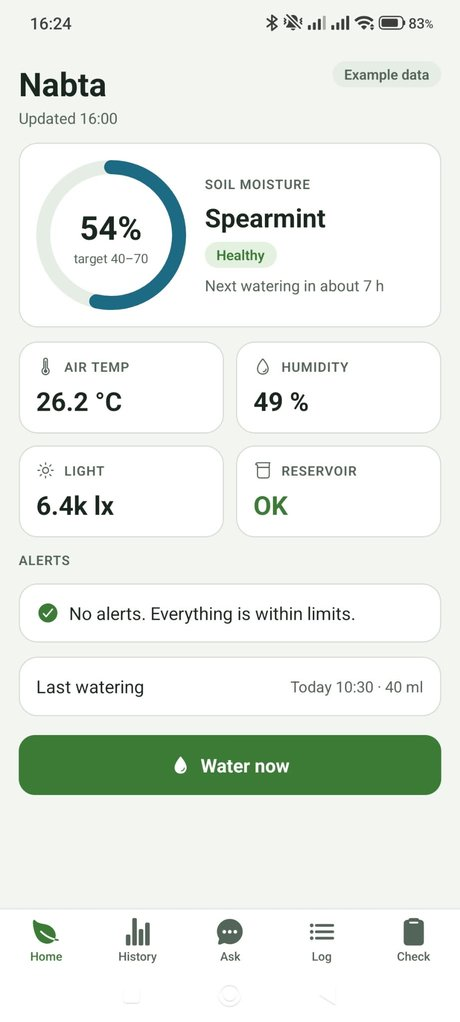
\includegraphics[width=\linewidth]{img/app_home.jpg}\caption{Home}\end{subfigure}\hfill
\begin{subfigure}[b]{0.188\textwidth}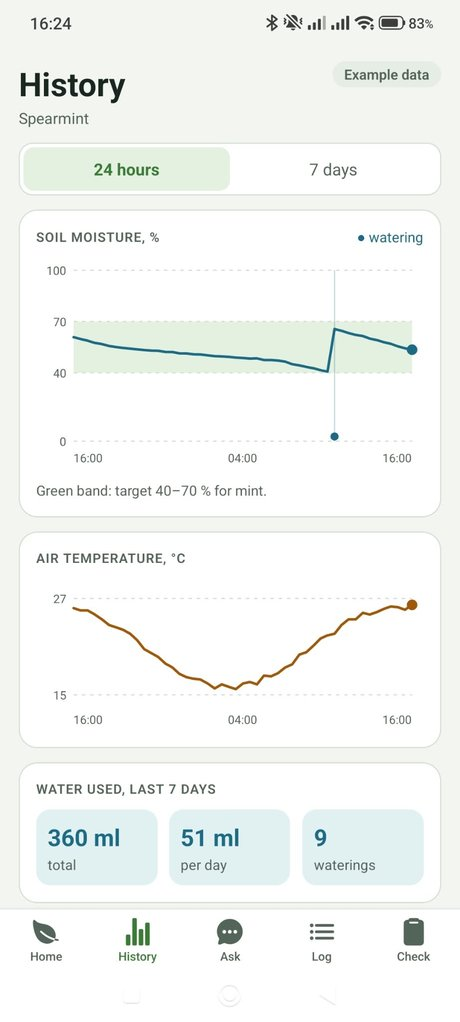
\includegraphics[width=\linewidth]{img/app_history.jpg}\caption{History}\end{subfigure}\hfill
\begin{subfigure}[b]{0.188\textwidth}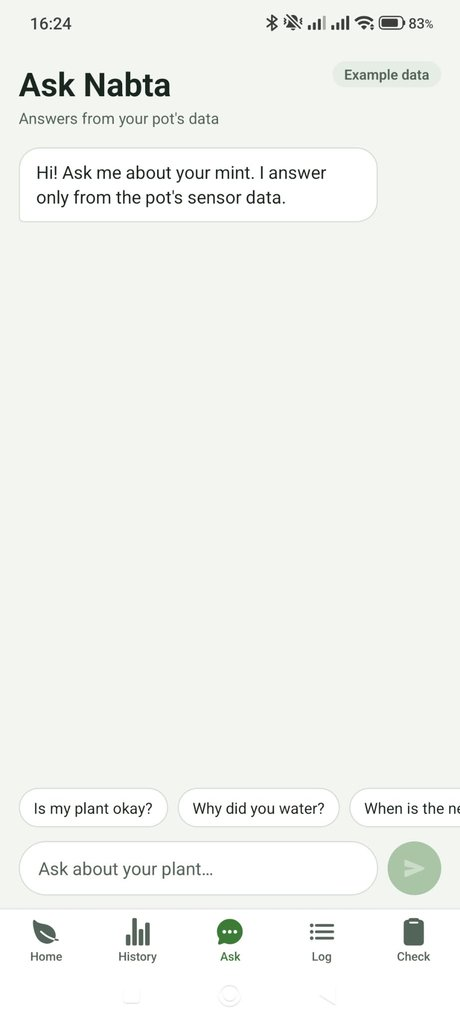
\includegraphics[width=\linewidth]{img/app_ask.jpg}\caption{Ask Nabta}\end{subfigure}\hfill
\begin{subfigure}[b]{0.188\textwidth}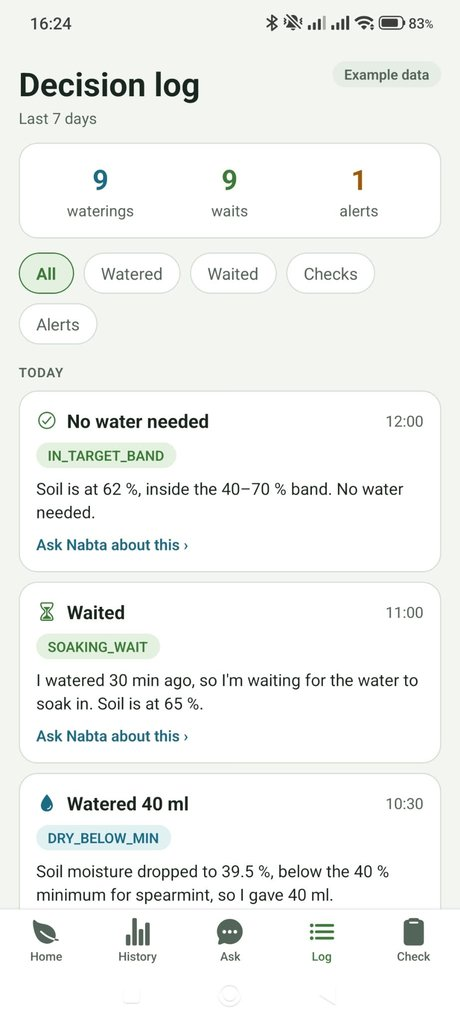
\includegraphics[width=\linewidth]{img/app_log.jpg}\caption{Decision log}\end{subfigure}\hfill
\begin{subfigure}[b]{0.188\textwidth}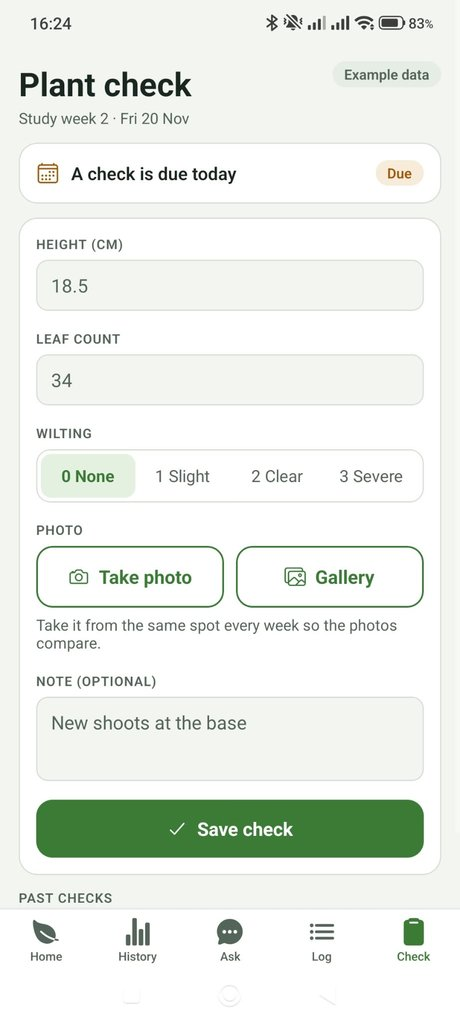
\includegraphics[width=\linewidth]{img/app_check.jpg}\caption{Plant check}\end{subfigure}
\caption{The Nabta app, showing example data.}
\end{figure}

\end{document}
